\documentclass[a4paper,11pt]{article}
\usepackage[brazil]{babel}
\usepackage[T1]{fontenc}
\usepackage{lmodern,booktabs,graphicx}
\pdfinfoomitdate=1
\pdftrailerid{}
\pdfsuppressptexinfo=15
\usepackage[a4paper,total={15.6cm,24.7cm},centering]{geometry}
\pagestyle{empty}
\begin{document}
\noindent\textbf{A01}\hfill {\small Prova A4 · largura útil de 15,6 cm}\par
\begin{figure}[!ht]
  \centering
  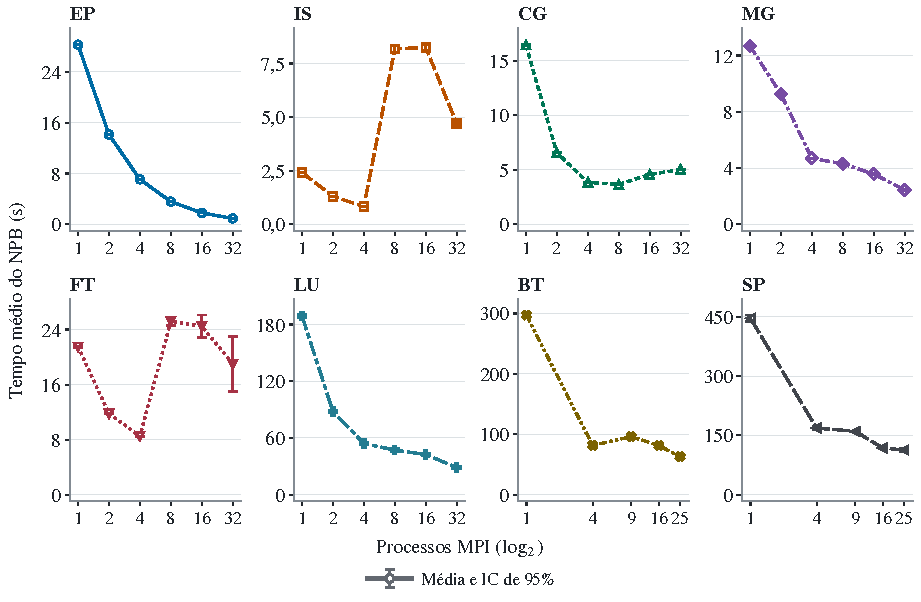
\includegraphics[width=\linewidth]{A01_tempo_medio_8paineis_4x2.pdf}
  \caption{Tempo médio do NPB por número de processos MPI. Barras de erro representam os ICs bilaterais de 95\% das médias. As escalas verticais são independentes.}
  \label{fig:a01}
\end{figure}

\clearpage

\noindent\textbf{C03}\hfill {\small Prova A4 · largura útil de 15,6 cm}\par
\begin{figure}[!ht]
  \centering
  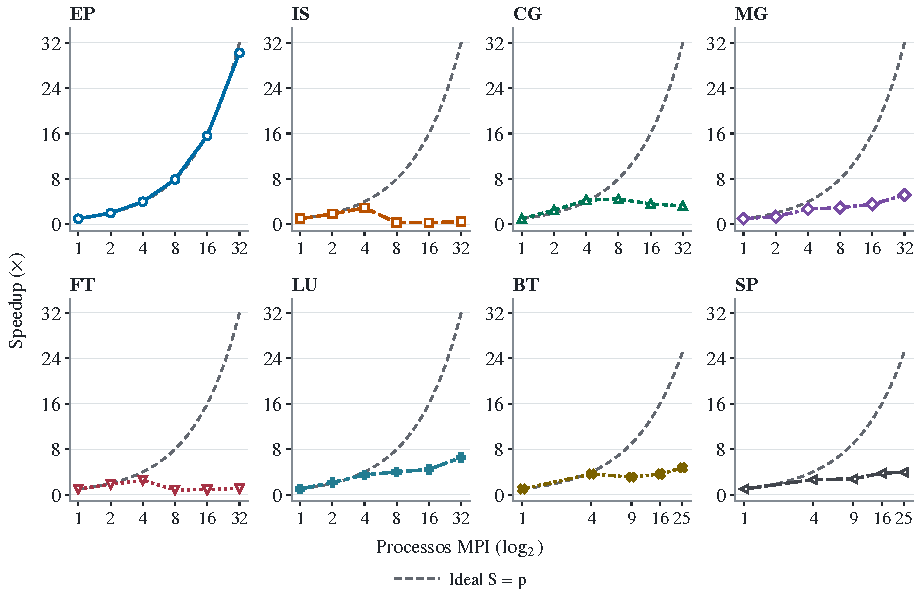
\includegraphics[width=\linewidth]{C03_speedup_8paineis_4x2.pdf}
  \caption{Speedup em relação à execução com um processo MPI. A linha tracejada representa o speedup ideal $S(p)=p$.}
  \label{fig:c03}
\end{figure}

\clearpage

\noindent\textbf{D03}\hfill {\small Prova A4 · largura útil de 15,6 cm}\par
\begin{figure}[!ht]
  \centering
  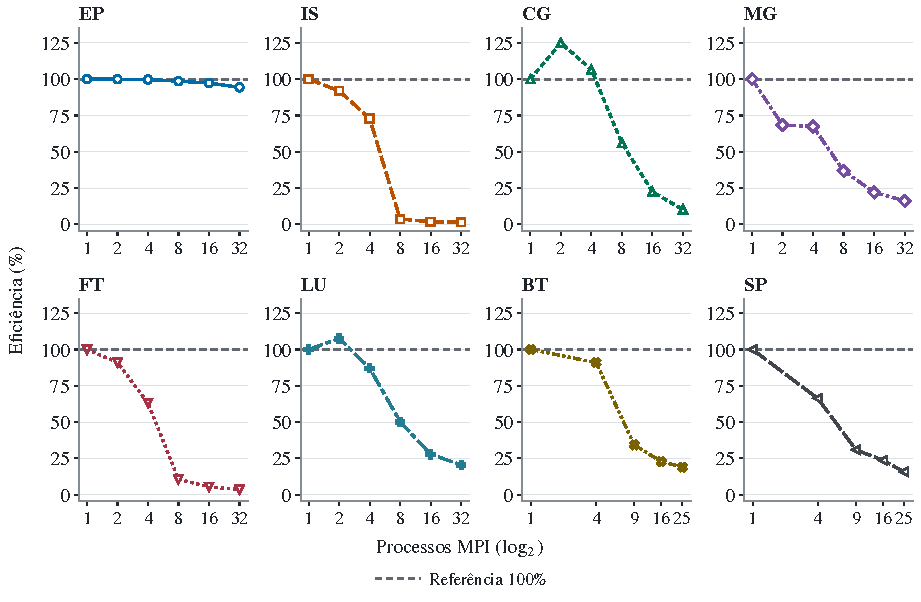
\includegraphics[width=\linewidth]{D03_eficiencia_8paineis_4x2.pdf}
  \caption{Eficiência paralela por quantidade de processos MPI. A linha tracejada indica o nível de referência de 100\%.}
  \label{fig:d03}
\end{figure}

\clearpage

\noindent\textbf{T01}\hfill {\small Prova A4 · largura útil de 15,6 cm}\par
\begin{table}[!ht]
  \centering
  \setlength{\belowcaptionskip}{5pt}
  \caption{Síntese do desempenho por benchmark.}
  \label{tab:sintese-desempenho}
  % Requer booktabs. Inserir com \input dentro de uma tabela centralizada.
\begingroup\small
\setlength{\tabcolsep}{2.5pt}%
\renewcommand{\arraystretch}{1.20}%
\begin{tabular*}{15.6cm}{@{\extracolsep{\fill}}lrrrrrr@{}}
\toprule
\shortstack[l]{Benchmark} & \shortstack[r]{Melhor $p$} & \shortstack[r]{Tempo médio\\mín. (s)} & \shortstack[r]{IC de 95\%\\(s)} & \shortstack[r]{Speedup\\máx. ($\times$)} & \shortstack[r]{Eficiência\\no melhor $p$ (\%)} & \shortstack[r]{Eficiência\\no maior $p$ (\%)} \\
\midrule
EP & 32 & 0,936 & [0,922 a 0,950] & 30,193 & 94,35 & 94,35 \\
IS & 4 & 0,826 & [0,819 a 0,833] & 2,918 & 72,94 & 1,60 \\
CG & 8 & 3,670 & [3,648 a 3,692] & 4,475 & 55,94 & 10,20 \\
MG & 32 & 2,444 & [2,421 a 2,467] & 5,189 & 16,21 & 16,21 \\
FT & 4 & 8,509 & [8,480 a 8,538] & 2,526 & 63,15 & 3,53 \\
LU & 32 & 28,857 & [28,757 a 28,957] & 6,556 & 20,49 & 20,49 \\
BT & 25 & 62,725 & [62,496 a 62,954] & 4,735 & 18,94 & 18,94 \\
SP & 25 & 113,178 & [108,876 a 117,480] & 3,946 & 15,78 & 15,78 \\
\bottomrule
\end{tabular*}%
\endgroup%

  \par\smallskip
  {\footnotesize\raggedright
    \textit{Nota.} Melhor $p$ é a configuração de menor tempo médio e o IC de 95\% refere-se a essa média. O maior $p$ avaliado é 25 para BT e SP e 32 para os demais benchmarks.\par}
\end{table}

\clearpage

\noindent\textbf{D03-2x4}\hfill {\small Prova A4 · largura útil de 15,6 cm}\par
\begin{figure}[!ht]
  \centering
  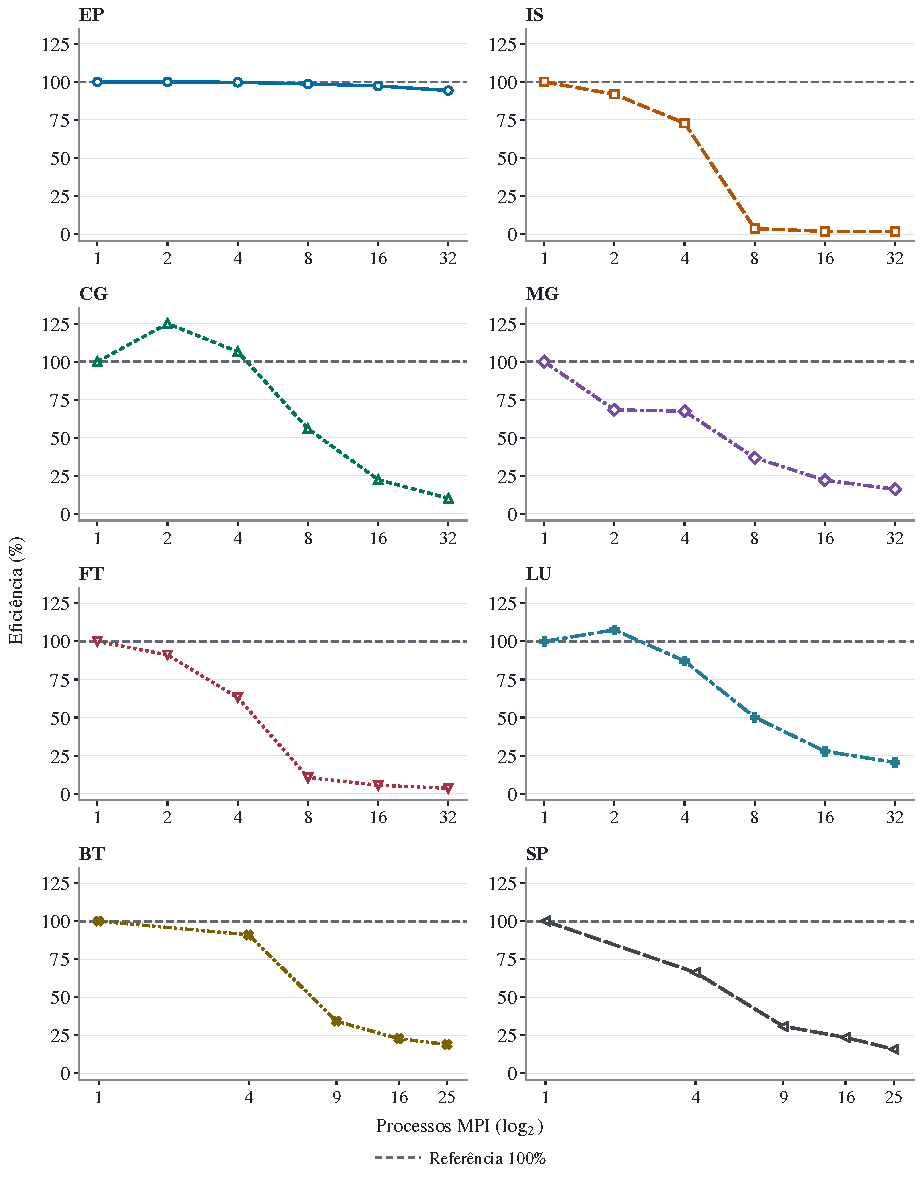
\includegraphics[width=\linewidth]{D03_eficiencia_8paineis_alternativa_2x4.pdf}
  \caption{Eficiência paralela na disposição 2×4. As escalas e os valores são os mesmos de D03.}
  \label{fig:d03-2x4}
\end{figure}
\end{document}
